\documentclass{beamer}

\usepackage{beamerthemeDresden}
\usepackage[frenchb]{babel}
\usepackage[utf8]{inputenc}
\usecolortheme{beaver}

\usepackage{listings}
\usepackage{xcolor}
\lstdefinestyle{base}{
  basicstyle=\ttfamily\color{black} \footnotesize,
  moredelim=**[is][\color{blue}]{@}{@},
  moredelim=**[is][\color{red}]{&}{&}
}

\setbeamertemplate{navigation symbols}{
\insertframenumber/
\inserttotalframenumber
}

\usepackage{color}
\definecolor{vert}{rgb}{0,0.5,0}
\definecolor{violet}{rgb}{0.5,0,0.5}

\usepackage{tikz}
\usetikzlibrary{calc,positioning,matrix,arrows,shapes.geometric,shapes.symbols,shapes.misc,shapes,automata,petri,decorations.markings,shadows}
\usepackage{array}
\usepackage{subfig}

\usepackage[absolute,overlay]{textpos}
\usepackage{tcolorbox}

%----------TIKZ
\usetikzlibrary{calc,arrows,shapes,automata,petri,positioning,decorations.markings,shadows}

\tikzset{
    use/.style={
    circle,draw=black,fill=black,scale=0.5,text=white
    },
    mpi/.style={
    rectangle,draw=black,fill=black,scale=0.8,text=white
    },
    provide/.style={
    circle,draw=black,fill=white,scale=0.5
    },
    component/.style={
    rectangle,rounded corners=3pt,draw=black
    },
    dcomponent/.style={
    rectangle,rounded corners=3pt,dashed,draw=black
    },
    progm/.style={rectangle,dashed, draw=black, thin, text width=10em, text centered,rounded corners, minimum height=2em},
  line/.style={draw, thin, ->, shorten >=2pt},
  purp/.style={rectangle, draw=violet,fill=violet!20, text width=10em, text centered,thin,rounded corners,inner sep=3pt},
  purp2/.style={rectangle, draw=violet,fill=violet!20, text width=15em, text centered,thin,rounded corners,inner sep=3pt},
}
%-------------

\def\pprec{\mathrel{\scalebox{.9}[1]{$\prec$}\mkern-3mu%
  \scalebox{.4}[1]{$\prec$}\mkern-5.5mu\scalebox{.4}[1]{$\prec$}}}

\makeatletter
    \newenvironment{withoutheadline}{
        \setbeamertemplate{headline}[default]
        \def\beamer@entrycode{\vspace*{-\headheight}}
    }{}
\makeatother

%-------------------------------------------------------------------
\title[From DSL to HPC Component-Based Runtime: A Multi-Stencil DSL Case Study]{From DSL to HPC Component-Based Runtime: A Multi-Stencil DSL Case Study}
\author[Julien Bigot (CEA), Hélène Coullon (INRIA), Christian Perez (INRIA)]{Julien Bigot, \underline{Hélène Coullon}, Christian Perez}
\institute[INRIA]{INRIA team Avalon\\Maison de la simulation (CEA)}
\date{WOLFHPC 2015 - $16^{th}$ November 2015}
%-------------------------------------------------------------------

\begin{document}

%---------------
%---------------
\begin{withoutheadline}

\begin{frame}
    \titlepage
\end{frame}

% INTRODUCTION / MOTIVATION
%-------------------------------------------------------------
\begin{frame}
\frametitle{Motivation} % HPC DSL
\begin{block}{+ Domain Specific Languages}
\begin{itemize}
\item Separation of concerns (domain/implementation)
\item Easy language for the user
\item Implicit optimizations
\item Implicit parallelization
\end{itemize}
\end{block}
\begin{alertblock}{- Domain Specific Languages}
\begin{itemize}
\item Difficulties deported to the DSL designer
\begin{itemize}
\item Low level high performance programming
\item Maintainability and portability
\end{itemize}
\item As many DSLs as domains
\begin{itemize}
\item DSL composition ?
\end{itemize}
\end{itemize}
\end{alertblock}
\end{frame}
%-------------------------------------------------------------
\begin{frame}
\frametitle{Motivation} % components
\begin{block}{Component models}
\begin{itemize}
\item Divide an application into several independent black boxes
\item Each component defines its interactions with outer world
\item Application = Assembly of components
\end{itemize}
\end{block}
\begin{block}{+ Component models}
\begin{itemize}
\item Maintainability through separation of concerns
\item Code-reuse and productivity
\item Dynamic assembly of components
\end{itemize}
\end{block}
\end{frame}
%-------------------------------------------------------------
\begin{frame}
\frametitle{Motivation} % components
\begin{tcolorbox}[width=\textwidth,title={Motivation}]
What if a DSL produces a component-based runtime ?
\begin{itemize}
\item Is it feasible ?
\item Is it efficient ?
\item Does it improve issues of DSLs ? (maintainability etc.)
\end{itemize}
\end{tcolorbox}

\begin{block}{Contributions}
\begin{itemize}
\item The Multi-Stencil Language (MSL)
\item A first component-based back end
\item No overheads introduced
\end{itemize}
\end{block}

\end{frame}
%-------------------------------------------------------------

% presentation of the table of contents
%-------------------------------------------------------------
\begin{frame}
\frametitle{Table of contents}
    \tableofcontents[hideallsubsections]
\end{frame}
%-------------------------------------------------------------

\end{withoutheadline}
%---------------
%---------------

%-------------------------------------------------------------
\section{Multi-Stencil Applications}
% related work, multi-stencil problem, language
%-------------------------------------------------------------
%----------------
\subsection{Multi-Stencil Applications}
%----------------
\begin{frame}
\frametitle{Numerical simulation = Multi-Stencil application}
\begin{center}
\resizebox{\textwidth}{!}{%
\begin{tikzpicture}
\def \n {5}
\def \radius {3cm}
\def \margin {8} % margin in angles, depends on the radius

  \node[purp2,align=center] (edp) at ({360/\n * (2 - 1)}:\radius) {Partial Differential Equations\\\scriptsize $\frac{\partial u(x,y,t)}{\partial t} = \frac{\partial^2 u(x,y,t)}{\partial x^2} + \frac{\partial^2 u(x,y,t)}{\partial y^2}$};
  \node[progm,align=center,right of=edp,node distance=6cm] (cond) {\scriptsize + specific behavior for\\\scriptsize boundary conditions};
  \path[line,dashed] (edp) -- (cond);
  \node[purp,align=center] (maillage) at ({360/\n * (1 - 1)}:\radius) {Mesh\\Time iterations};
  \path[->] (maillage) edge[<-,thin,shorten <=2pt,shorten >=2pt, bend right=40]  node [fill=white,align=center] {\scriptsize Time and space\\\scriptsize discretization} (edp.east);
  \path[] (edp.west) edge[thin,shorten <=2pt,shorten >=2pt, bend right=90]  node [draw,circle,fill=white] (plus) {\scriptsize +} (maillage.west);
  \node[purp,align=center, below of=plus, node distance=3.5cm] (sche) {Explicit\\numerical schemes\\\textcolor{red}{stencils}};
  \node[progm,align=center,right of=sche,node distance=5.5cm] (expl) {\scriptsize Step by step approximation of the phenomena};
  \path[line,dashed] (sche) -- (expl);
  \path[line] (plus) -- node [fill=white,align=center] {\scriptsize Numerical methods\\\scriptsize Finite difference/volume/elment} (sche);
\end{tikzpicture}
}
\end{center}
\end{frame}
%----------------

%----------------
\begin{frame}
\frametitle{Time and Mesh}
\begin{block}{Time}
At each time iteration of the simulation are applied the \emph{computation kernels} of the application.
\end{block}
\begin{block}{Mesh}
\begin{itemize}
\item A Mesh is a connected undirected graph $\mathcal{M}=(V,E)$ without bridges
\item Mesh entities are a subset of $V \cup E$
\end{itemize}
\end{block}
\begin{center}
\resizebox{6cm}{!}{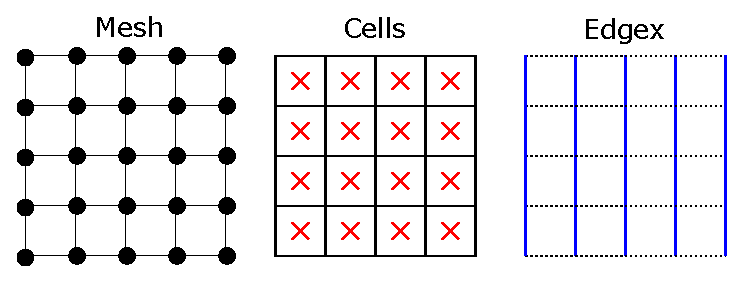
\includegraphics{./images/mesh.pdf}}
\end{center}
\end{frame}
%----------------

%----------------
\begin{frame}
\frametitle{Data and Computation Kernels}
\begin{block}{Data}
Data is a set of numerical values, each one attached to a given mesh entity
\end{block}
\begin{block}{Computation kernel}
\begin{itemize}
\item Set of data read for the computation
\begin{itemize}
\item Each one associated to a stencil shape
\end{itemize}
\item Data written by the computation
\item A numerical expression
\item A computation domain
\begin{itemize}
\item Subset of mesh entities
\end{itemize}
\end{itemize}
\end{block}
\end{frame}
%----------------

%----------------
% \begin{frame}
% \frametitle{Computation kernel: Examples}
% \begin{center}
% \resizebox{6cm}{!}{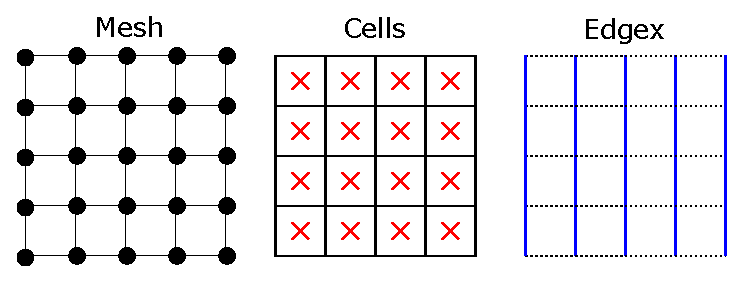
\includegraphics{./images/mesh.pdf}}
% \hspace{10pt}
% \resizebox{5cm}{!}{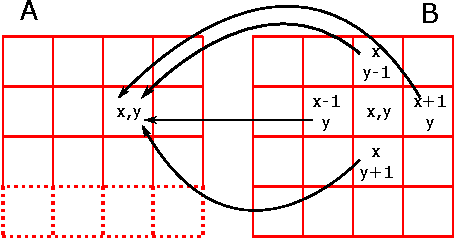
\includegraphics{./images/stencil1.pdf}}
% \end{center}
% Compute $A$ using $\{(B,n1)\}$ on the computation domain called $dc1$ with the numerical expression
% \tiny
% \begin{equation*}
% A(x,y)=B(x+1,y)+B(x-1,y)+B(x,y+1)+B(x,y-1).
% \end{equation*}
% \end{frame}
%----------------

%----------------
% \begin{frame}
% \frametitle{Computation kernel: Example}
% \begin{center}
% \resizebox{6cm}{!}{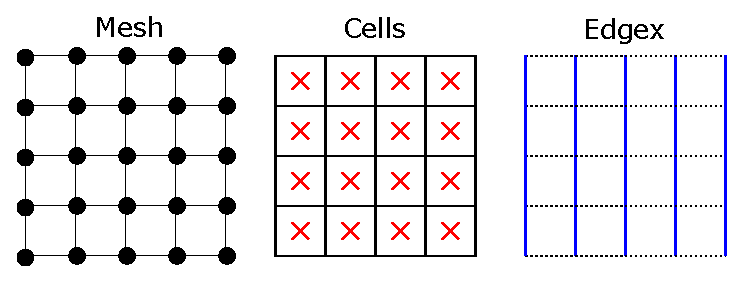
\includegraphics{./images/mesh.pdf}}
% \hspace{10pt}
% \resizebox{5cm}{!}{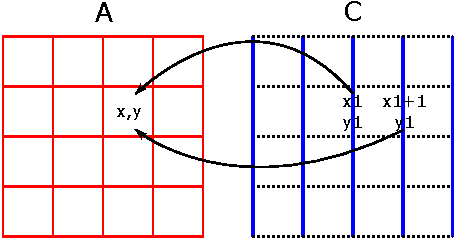
\includegraphics{./images/stencil2.pdf}}
% \end{center}
% \end{frame}
%----------------

%----------------
\begin{frame}
\frametitle{Multi-Stencil application}
\begin{center}
$\mathcal{MSP}(T,\mathcal{M},\mathcal{E},\mathcal{D},\Delta,\Gamma)$
\end{center}
\begin{itemize}
\item $T$ the set of time iterations to tun the simulation
\item $\mathcal{M}$ the mesh of the simulation
\item $\mathcal{E}$ the set of mesh entities
\item $\mathcal{D}$ the set of computation domains
\item $\Delta$ the set of data
\item $\Gamma$ the set of computations
\end{itemize}
\center \textit{= the six sections of a \emph{Multi-Stencil Language} program !}
\end{frame}
%----------------

%-------------------------------------------------------------
\section{MSL Overview}
% take the same notations inside components + user
%-------------------------------------------------------------
\subsection{MSL Overview}

%----------------
\begin{frame}[fragile]
\frametitle{Example}
\begin{columns}
\begin{column}{.52\textwidth}
\resizebox{\textwidth}{!}{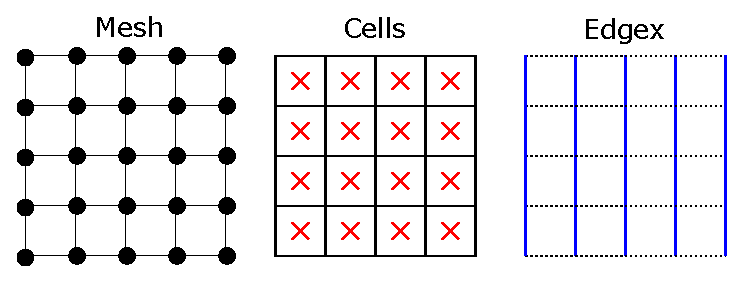
\includegraphics{./images/mesh.pdf}}
\hspace{10pt}
\resizebox{\textwidth}{!}{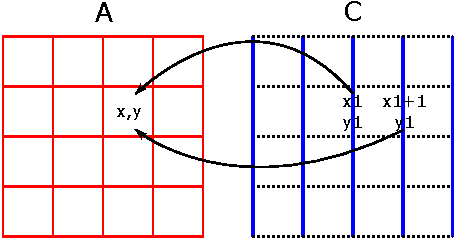
\includegraphics{./images/stencil2.pdf}}
\end{column}
\begin{column}{.48\textwidth}
$\mathcal{MSP}(T,\mathcal{M},\mathcal{E},\mathcal{D},\Delta,\Gamma)$\\

\medskip
\textit{\textcolor{blue}{blue} = MSL and black = user identifiers}

\medskip
\begin{lstlisting}[style=base]
@mesh:@ cart
@mesh entities:@ cell@,@edgex
@computation domains:@
  allcell @in@ cell
  alledgex @in@ edgex
@data:@
  A@,@cell
  C@,@edgex
@time:@500
@computations:@
  A@[@allcell@]@=&comp&@(@C@[@n1@]@@)@
\end{lstlisting}
\end{column}
\end{columns}
\end{frame}

%----------------
\begin{frame}[fragile]
\frametitle{Where is the code ?}
Keywords + identifiers ? That's it ? Where is the code ???
\end{frame}

%----------------
\begin{frame}[fragile]
\frametitle{Where is the code ?}
\begin{block}{Data parallelism}
Whatever the mesh is and the exact computations are:
\begin{itemize}
\item mesh and data are splitted among resources
\item synchronizations detected from \textbf{computation dependencies}
\end{itemize}
\end{block}

\begin{block}{Mid-grain task parallelism}
Task = complete computation\\
Whatever the mesh is and the exact computations are:
\begin{itemize}
\item task dependencies detected from \textbf{computation dependencies}
\end{itemize}
\end{block}

\begin{alertblock}{Fine grain optimizations and parallelizations}
Stencil compilers already exist !
\end{alertblock}

\end{frame}


%----------------
\begin{frame}[fragile]
\frametitle{Where is the code ?}
\begin{block}{Data parallelism}
Whatever the mesh is and the exact computations are:
\begin{itemize}
\item mesh and data are splitted among resources
\item synchronizations detected from computation dependencies
\end{itemize}
\end{block}

\begin{block}{Mid-grain task parallelism}
Task = complete computation\\
Whatever the mesh is and the exact computations are:
\begin{itemize}
\item task dependencies detected from computation dependencies
\end{itemize}
\end{block}

\begin{alertblock}{Fine grain optimizations and parallelizations}
Stencil compilers already exist !
\end{alertblock}

\begin{textblock*}{0.8\textwidth}(20mm,32mm)
\begin{tcolorbox}[width=\textwidth,title={MSL = computation dependencies}]
  \begin{itemize}  
  \item produces a component based parallel scheduling of the simulation
  \item it is agnostic from the mesh
  \item it is agnostic from the actual numerical code
  \end{itemize}
\end{tcolorbox} 
\end{textblock*}
% based parallel scheduling of the simulation\\ It is agnostic from the mesh\\it is agnostic from the actual numerical code

\end{frame}

% %----------------
% \begin{frame}[fragile]
% \frametitle{MSL Example}
% \begin{columns}
% \begin{column}{.52\textwidth}
% \begin{lstlisting}[style=base]
% @mesh:@ cart
% @mesh entities:@ cell,edgex,edgey
% @computation domains:@
%   allcell in cell
%   alledgex in edgex
%   alledgey in edgey
%   part1edgex in edgex
%   part2edgex in edgex
% @data:@
%   a,cell
%   b,cell
%   c,edgex
%   d,edgex
%   e,edgey
% \end{lstlisting}
% \end{column}
% \begin{column}{.48\textwidth}
% \begin{lstlisting}[style=base]
%   f,cell
%   g,edgey
%   h,edgex
%   i,cell
%   j,edgex
% @time:@500
% @computations:@
%   b[allcell]=&c0&(a)
%   c[alledgex]=&c1&(b[n1])
%   d[alledgex]=&c2&(c)
%   e[alledgey]=&c3&(c)
%   f[allcell]=&c4&(d[n1])
%   g[alledgey]=&c5&(e)
%   h[alledgex]=&c6&(f)
%   i[allcell]=&c7&(g,h)
%   j[partedgex]=&c8&(i[n1])
% \end{lstlisting}
% \end{column}
% \end{columns}
% \end{frame}
% %----------------

% %----------------
% \begin{frame}
% \frametitle{Multi-Stencil Language}
% \begin{alertblock}{MSL is not}
% \begin{itemize}
% \item a new stencil optimizer/compiler
% \item a new distributed data structure
% \end{itemize}
% \end{alertblock}
% \begin{block}{MSL is}
% \begin{itemize}
% \item a high-level language for multi-stencil simulations
% \item agnostic from the type of mesh used (data structure)
% \end{itemize}
% \end{block}
% \begin{center}
% \textit{MSL produces an empty\\component-based parallel scheduling of the simulation}
% \end{center}
% \end{frame}
% %----------------

%----------------
\begin{frame}
\frametitle{Related Work}
\begin{block}{Complementary work}
\begin{itemize}
\item Distributed data structures: SkelGIS, Global Arrays
\item Stencil DSLs (on grids): Pochoir, PATUS
\item Stencil DSLs (on unstructured meshes): OP2, Liszt
\end{itemize}
\end{block}
\begin{alertblock}{Similar work}
\begin{itemize}
\item Pipeline of stencil computations for image processing: Halide
\begin{itemize}
\item On grids (image), different abstraction level
\end{itemize}
\item DSL to component-based runtime ?
\end{itemize}
\end{alertblock}
\end{frame}
%----------------
%-------------------------------------------------------------

% %----------------
% \begin{frame}
% \frametitle{MSL to Component-based runtime}
% \begin{block}{Ready-to-fill parallel scheduling: mid-grain parallelism}
% \begin{itemize}
% \item Data parallelism
% \begin{itemize}
% \item External distributed data structure
% \item Automatic detection of synchronizations
% \end{itemize}
% \item Task parallelism
% \begin{itemize}
% \item Compile a static scheduling of computation kernels
% \end{itemize}
% \end{itemize}
% \end{block}
% The fine grain parallelism is left to other languages: 
% \begin{itemize}
% \item OpenMP in the kernels
% \item Kernels generated by stencil compilers for CPU or GPU (Pochoir, Liszt etc.)
% \end{itemize}
% \end{frame}
% %----------------

%----------------
% \begin{frame}
% \frametitle{MSL to Component-based runtime}
% \begin{block}{Empty component-based parallel scheduling of the simulation}
% \begin{itemize}
% \item Data parallelism
% \begin{itemize}
% \item Use of an external distributed data structure
% \item Automatic detection of synchronizations
% \end{itemize}
% \item Mid-grain task parallelism
% \begin{itemize}
% \item A task is a complete computation (space loop)
% \end{itemize}
% \end{itemize}
% \end{block}
% The fine grain optimizations/parallelizations are left to other languages: 
% \begin{itemize}
% \item OpenMP in the kernels
% \item Kernels generated by stencil compilers (Pochoir, Liszt etc.)
% \end{itemize}
% \end{frame}
%----------------

%----------------
\begin{frame}
\frametitle{MSL to Component-based runtime}
\begin{center}
$\mathcal{MSP}(T,\mathcal{M},\mathcal{E},\mathcal{D},\Delta,\Gamma)$\\

\bigskip
\begin{tikzpicture}[remember picture]
  \node[rectangle,rounded corners=3pt,thick,inner sep=5pt,draw=black,dotted] (proc) {
    \begin{tikzpicture}[shorten >=1pt, node distance=2cm, on grid, auto]
     \node[component,solid,draw=red] (D) at (0,0) {$Driver$};
     \node[provide,scale=0.5,solid] (Dp) at (-1,0) {};
     \node[solid] (Ds) at (-1.5,0) {start};
     \node[use,scale=0.5,solid,right=1.5cm of D] (Du1) {};
     \node[use,scale=0.5,solid,below=1.75cm of D] (Du2) {};
     \node[use,scale=0.5,solid,below=0.8cm of Du1] (Du3) {$m$};

     \node[provide,scale=0.5,solid,below=0.15 of Du2] (Tp) {};
     \node[component,solid,below=1.6cm of Tp] (T) {$Time$};
     \node[use,scale=0.5,solid,right=1cm of T] (Tu) {};
     \node[solid,left=0.8cm of T] (tt) {$T$};

     \node[provide,scale=0.5,solid,right=0.15 of Tu] (Cp) {};
     \node[component,dashed,right=2cm of Cp] (C) {$Computations$};
     \node[use,scale=0.5,solid,above=0.8cm of C] (Cu) {};
     \node[solid,right=0.2cm of Cu] (star) {$*$};
     \node[solid,right=1.5cm of C] (gamma) {$\Gamma$};

     \node[provide,scale=0.5,solid,below right=0.2 of Du3] (Datap1) {};
     \node[provide,scale=0.5,solid,above=0.15 of Cu] (Datap2) {};
     \node[component,solid,double,above=0.8cm of Datap2] (Data) {$Data$};
     \node[use,scale=0.5,solid,above=0.8cm of Data] (Datau) {};
     \node[solid,left=1cm of Data] (delta) {$\Delta,\mathcal{D}$};
     %\node[mpi,scale=0.8,rounded corners=0pt,solid,right=1cm of Data] (mpidata) {};
     %\node[solid,above=0.2cm of mpidata] (star2) {$*$};

     \node[provide,scale=0.5,solid,right=0.15 of Du1] (DDSp1) {};
     \node[provide,scale=0.5,solid,above=0.15 of Datau] (DDSp2) {};
     \node[component,solid,above=0.8cm of DDSp2] (DDS) {$DDS$};
     \node[solid,right=1.2cm of DDS] (m) {$\mathcal{M},\mathcal{E}$};
   
    \path[-]
      (Dp) edge [solid] node {} (D)
      (D) edge [solid] node {} (Du1)
          edge [solid] node {} (Du2)
          edge [solid] node {} (Du3)
      (DDSp1) edge [solid] node {} (DDS)
      (Tp) edge [solid] node {} (T)
      (T)  edge [solid] node {} (Tu)
      (Cp) edge [solid] node {} (C)
      (C) edge [solid] node {} (Cu)
      (Datap2) edge [solid] node {} (Data)
      (Datap1) edge [solid] node {} (Data)
      (Data) edge [solid] node {} (Datau)
      (DDSp2) edge [solid] node {} (DDS);
    \end{tikzpicture}
    };
    \node[mpi,scale=0.8,rounded corners=0pt,solid,right=0.5cm of proc] (mpidata) {};
    \node[solid,above=0.1cm of mpidata] (star2) {$*$};
    \node[solid,below=2.5cm of proc.west,anchor=west] (core) {\textit{\tiny{Duplicated on each processor/core}}};
    \path[-]
      (Data.east) edge node {} (mpidata);
  \end{tikzpicture}
\end{center}
\end{frame}
%-------------------------------------------------------------

%----------------
\begin{frame}
\frametitle{MSL to Component-based runtime}
\begin{center}
$\mathcal{MSP}(T,\mathcal{M},\mathcal{E},\mathcal{D},\Delta,\Gamma)$\\

\bigskip
\begin{tikzpicture}[remember picture]
  \node[rectangle,rounded corners=3pt,thick,inner sep=5pt,draw=red,dotted] (proc) {
    \begin{tikzpicture}[shorten >=1pt, node distance=2cm, on grid, auto]
     \node[component,solid] (D) at (0,0) {$Driver$};
     \node[provide,scale=0.5,solid] (Dp) at (-1,0) {};
     \node[solid] (Ds) at (-1.5,0) {start};
     \node[use,scale=0.5,solid,right=1.5cm of D] (Du1) {};
     \node[use,scale=0.5,solid,below=1.75cm of D] (Du2) {};
     \node[use,scale=0.5,solid,below=0.8cm of Du1] (Du3) {$m$};

     \node[provide,scale=0.5,solid,below=0.15 of Du2] (Tp) {};
     \node[component,solid,below=1.6cm of Tp] (T) {$Time$};
     \node[use,scale=0.5,solid,right=1cm of T] (Tu) {};
     \node[solid,left=0.8cm of T] (tt) {$T$};

     \node[provide,scale=0.5,solid,right=0.15 of Tu] (Cp) {};
     \node[component,dashed,right=2cm of Cp] (C) {$Computations$};
     \node[use,scale=0.5,solid,above=0.8cm of C] (Cu) {};
     \node[solid,right=0.2cm of Cu] (star) {$*$};
     \node[solid,right=1.5cm of C] (gamma) {$\Gamma$};

     \node[provide,scale=0.5,solid,below right=0.2 of Du3] (Datap1) {};
     \node[provide,scale=0.5,solid,above=0.15 of Cu] (Datap2) {};
     \node[component,solid,draw=red,double,above=0.8cm of Datap2] (Data) {$Data$};
     \node[use,scale=0.5,solid,above=0.8cm of Data] (Datau) {};
     \node[solid,left=1cm of Data] (delta) {$\Delta,\mathcal{D}$};
     %\node[mpi,scale=0.8,rounded corners=0pt,solid,right=1cm of Data] (mpidata) {};
     %\node[solid,above=0.2cm of mpidata] (star2) {$*$};

     \node[provide,scale=0.5,solid,right=0.15 of Du1] (DDSp1) {};
     \node[provide,scale=0.5,solid,above=0.15 of Datau] (DDSp2) {};
     \node[component,draw=red,solid,above=0.8cm of DDSp2] (DDS) {$DDS$};
     \node[solid,right=1.2cm of DDS] (m) {$\mathcal{M},\mathcal{E}$};
   
    \path[-]
      (Dp) edge [solid] node {} (D)
      (D) edge [solid] node {} (Du1)
          edge [solid] node {} (Du2)
          edge [solid] node {} (Du3)
      (DDSp1) edge [solid] node {} (DDS)
      (Tp) edge [solid] node {} (T)
      (T)  edge [solid] node {} (Tu)
      (Cp) edge [solid] node {} (C)
      (C) edge [solid] node {} (Cu)
      (Datap2) edge [solid] node {} (Data)
      (Datap1) edge [solid] node {} (Data)
      (Data) edge [solid] node {} (Datau)
      (DDSp2) edge [solid] node {} (DDS);
    \end{tikzpicture}
    };
    \node[mpi,scale=0.8,rounded corners=0pt,solid,right=0.5cm of proc] (mpidata) {};
    \node[solid,above=0.1cm of mpidata] (star2) {$*$};
    \node[solid,below=2.5cm of proc.west,anchor=west] (core) {\textit{\tiny{Duplicated on each processor/core}}};
    \path[-]
      (Data.east) edge node {} (mpidata);
  \end{tikzpicture}
\end{center}
\end{frame}
%-------------------------------------------------------------

%----------------
\begin{frame}
\frametitle{MSL to Component-based runtime}
\begin{center}
$\mathcal{MSP}(T,\mathcal{M},\mathcal{E},\mathcal{D},\Delta,\Gamma)$\\

\bigskip
\begin{tikzpicture}[remember picture]
  \node[rectangle,rounded corners=3pt,thick,inner sep=5pt,draw=black,dotted] (proc) {
    \begin{tikzpicture}[shorten >=1pt, node distance=2cm, on grid, auto]
     \node[component,solid] (D) at (0,0) {$Driver$};
     \node[provide,scale=0.5,solid] (Dp) at (-1,0) {};
     \node[solid] (Ds) at (-1.5,0) {start};
     \node[use,scale=0.5,solid,right=1.5cm of D] (Du1) {};
     \node[use,scale=0.5,solid,below=1.75cm of D] (Du2) {};
     \node[use,scale=0.5,solid,below=0.8cm of Du1] (Du3) {$m$};

     \node[provide,scale=0.5,solid,below=0.15 of Du2] (Tp) {};
     \node[component,solid,draw=red,below=1.6cm of Tp] (T) {$Time$};
     \node[use,scale=0.5,solid,right=1cm of T] (Tu) {};
     \node[solid,left=0.8cm of T] (tt) {$T$};

     \node[provide,scale=0.5,solid,right=0.15 of Tu] (Cp) {};
     \node[component,dashed,draw=red,right=2cm of Cp] (C) {$Computations$};
     \node[use,scale=0.5,solid,above=0.8cm of C] (Cu) {};
     \node[solid,right=0.2cm of Cu] (star) {$*$};
     \node[solid,right=1.5cm of C] (gamma) {$\Gamma$};

     \node[provide,scale=0.5,solid,below right=0.2 of Du3] (Datap1) {};
     \node[provide,scale=0.5,solid,above=0.15 of Cu] (Datap2) {};
     \node[component,solid,double,above=0.8cm of Datap2] (Data) {$Data$};
     \node[use,scale=0.5,solid,above=0.8cm of Data] (Datau) {};
     \node[solid,left=1cm of Data] (delta) {$\Delta,\mathcal{D}$};
     %\node[mpi,scale=0.8,rounded corners=0pt,solid,right=1cm of Data] (mpidata) {};
     %\node[solid,above=0.2cm of mpidata] (star2) {$*$};

     \node[provide,scale=0.5,solid,right=0.15 of Du1] (DDSp1) {};
     \node[provide,scale=0.5,solid,above=0.15 of Datau] (DDSp2) {};
     \node[component,solid,above=0.8cm of DDSp2] (DDS) {$DDS$};
     \node[solid,right=1.2cm of DDS] (m) {$\mathcal{M},\mathcal{E}$};
   
    \path[-]
      (Dp) edge [solid] node {} (D)
      (D) edge [solid] node {} (Du1)
          edge [solid] node {} (Du2)
          edge [solid] node {} (Du3)
      (DDSp1) edge [solid] node {} (DDS)
      (Tp) edge [solid] node {} (T)
      (T)  edge [solid] node {} (Tu)
      (Cp) edge [solid] node {} (C)
      (C) edge [solid] node {} (Cu)
      (Datap2) edge [solid] node {} (Data)
      (Datap1) edge [solid] node {} (Data)
      (Data) edge [solid] node {} (Datau)
      (DDSp2) edge [solid] node {} (DDS);
    \end{tikzpicture}
    };
    \node[mpi,scale=0.8,rounded corners=0pt,solid,right=0.5cm of proc] (mpidata) {};
    \node[solid,above=0.1cm of mpidata] (star2) {$*$};
    \node[solid,below=2.5cm of proc.west,anchor=west] (core) {\textit{\tiny{Duplicated on each processor/core}}};
    \path[-]
      (Data.east) edge node {} (mpidata);
  \end{tikzpicture}
\end{center}
\end{frame}
%-------------------------------------------------------------

%-------------------------------------------------------------
\section{Compiler}
% A slide example MS, 6 slides on graph transformations
%-------------------------------------------------------------
\subsection{Compiler}
%----------------
\begin{frame}[fragile]
\frametitle{Example}
\begin{columns}
\begin{column}{.52\textwidth}
\begin{lstlisting}[style=base]
@mesh:@ cart
@mesh entities:@ cell,edgex,edgey
@computation domains:@
  allcell @in@ cell
  alledgex @in@ edgex
  alledgey @in@ edgey
  part1edgex @in@ edgex
  part2edgex @in@ edgex
@data:@
  a,cell
  b,cell
  c,edgex
  d,edgex
  e,edgey
\end{lstlisting}
\end{column}
\begin{column}{.48\textwidth}
\begin{lstlisting}[style=base]
  f,cell
  g,edgey
  h,edgex
  i,cell
  j,edgex
@time:@500
@computations:@
  b[allcell]=&c0&(a)
  c[alledgex]=&c1&(b[n1])
  d[alledgex]=&c2&(c)
  e[alledgey]=&c3&(c)
  f[allcell]=&c4&(d[n1])
  g[alledgey]=&c5&(e)
  h[alledgex]=&c6&(f)
  i[allcell]=&c7&(g,h)
  j[partedgex]=&c8&(i[n1])
\end{lstlisting}
\end{column}
\end{columns}
\end{frame}
%----------------

%----------------
\begin{frame}
\frametitle{Data parallelism}
\begin{enumerate}
\item Assembly of components duplicated on each resource (SPMD)
\item External Distributed Data Structure to split data among resources
\item Detect when synchronizations are needed
\end{enumerate}

\medskip
\begin{block}{Synchronization}
When a computation read a data, using a stencil shape, that has been written by a previous computation.
\end{block}

$\Gamma = [c_0,c_1,c_2,c_3,c_4,c_5,c_6,c_7,c_8]$\\
$\hookrightarrow [c_0,sync_1,c_1,c_2,c_3,sync_4,c_4,c_5,c_6,c_7,sync_8,c_8]$
\end{frame}
%----------------

%----------------
\begin{frame}
\frametitle{Data and task parallelism}

\begin{block}{Dependency graph}
\begin{enumerate}
\item Each node is a computation or a synchronization
\item Each edge is a dependency: a computation read a data that has been written before.
\end{enumerate}
\end{block}

\begin{center}
\begin{tikzpicture}[shorten >=1pt, node distance=2cm, on grid, auto]
   \node (c0) at (0,0) {$c_0$};
   \node[right=1 of c0] (sy1) {$sync_1$};
   \node[right=1 of sy1] (c1) {$c_1$};
   \node[above right=1 of c1] (c2) {$c_2$};
   \node[below right=1 of c1] (c3) {$c_3$};
   \node[right=1 of c2] (sy4) {$sync_4$};
   \node[right=1 of c3] (c5) {$c_5$};
   \node[right=1 of sy4] (c4) {$c_4$};
   \node[right=1 of c4] (c6) {$c_6$};
   \node[below right=1 of c6] (c7) {$c_7$};
   \node[right=1 of c7] (sy8) {$sync_8$};
   \node[right=1 of sy8] (c8) {$c_8$};
 
  \path[->]
    (c0) edge node {} (sy1)
    (sy1) edge node {} (c1)
    (c1)  edge node {} (c2)
          edge node {} (c3)
    (c2) edge node {} (sy4)
    (sy4) edge node {} (c4)
    (c4) edge node {} (c6)
    (c3) edge node {} (c5)
    (c5) edge node {} (c7)
    (c6) edge node {} (c7)
    (c7) edge node {} (sy8)
    (sy8) edge node {} (c8);
\end{tikzpicture}
\end{center}

\begin{center}
\textcolor{gray}{Dynamic} or static scheduling ?
\end{center}
\end{frame}
%----------------

%----------------
% \begin{frame}
% \frametitle{Which scheduling ?}
% From the dependency graph we can:
% \begin{itemize}
% \item Use a dynamic scheduler
% \item Compute a static scheduling
% \end{itemize}

% In this work,
% \begin{itemize}
% \item We build a static scheduling of the multi-stencil application
% \item This static scheduling can be dumped to a component-based runtime
% \end{itemize}
% \end{frame}
%----------------

%----------------
\begin{frame}
\frametitle{Series-Parallel Tree}
\small\textit{Valdes \& Al, The Recognition of Series Parallel Digraphs, STOC '79}
\normalsize
\begin{columns}
\begin{column}{.48\textwidth}
\begin{center}
\resizebox{\textwidth}{!}{%
\begin{tikzpicture}[shorten >=1pt, node distance=2cm, on grid, auto]
   \node[] (s0)    at (0,0) {$\mathcal{S}$};
   
   \node[] (c0)    at (-3,1) {$c_0$};
   \node[] (star1) at (-2,1) {$sync_1$};
   \node[] (c1)    at (-1,1) {$c_1$};
   \node[] (p0)    at ( 0,1) {$\mathcal{P}$};
   \node[] (c7)    at ( 1,1) {$c_7$};
   \node[] (star8) at ( 2,1) {$sync_8$};
   \node[] (c8)    at ( 3,1) {$c_8$};

   \node[] (s1)    at (-1,2) {$\mathcal{S}$};
   \node[] (s2)    at (1,2) {$\mathcal{S}$};
   
   \node[] (c2)    at (-3,3) {$c_2$};
   \node[] (star4) at (-2,3) {$sync_4$};
   \node[] (c4)    at (-1,3) {$c_4$};
   \node[] (c6)    at ( 0,3) {$c_6$};
   \node[] (c3)    at ( 1,3) {$c_3$};
   \node[] (c5)    at ( 2,3) {$c_5$};

 
  \path[->]
    (s0) edge node {} (c0)
         edge node {} (star1)
         edge node {} (c1)
         edge node {} (p0)
         edge node {} (c7)
         edge node {} (star8)
         edge node {} (c8)
    (p0) edge node {} (s1)
         edge node {} (s2)
    (s1) edge node {} (c2)
         edge node {} (star4)
         edge node {} (c4)
         edge node {} (c4)
         edge node {} (c6)
    (s2) edge node {} (c3)
         edge node {} (c5);
  \end{tikzpicture}
  }
\end{center}
\end{column}
\begin{column}{.52\textwidth}

\end{column}
\end{columns}
\end{frame}
%----------------

%----------------
\begin{frame}
\frametitle{Series-Parallel Tree}
\small\textit{Valdes \& Al, The Recognition of Series Parallel Digraphs, STOC '79}
\normalsize
\begin{columns}
\begin{column}{.48\textwidth}
\begin{center}
\resizebox{\textwidth}{!}{%
\begin{tikzpicture}[shorten >=1pt, node distance=2cm, on grid, auto]
   \node[] (s0)    at (0,0) {$\mathcal{S}$};
   
   \node[] (c0)    at (-3,1) {$c_0$};
   \node[] (star1) at (-2,1) {$sync_1$};
   \node[] (c1)    at (-1,1) {$c_1$};
   \node[] (p0)    at ( 0,1) {$\mathcal{P}$};
   \node[] (c7)    at ( 1,1) {$c_7$};
   \node[] (star8) at ( 2,1) {$sync_8$};
   \node[] (c8)    at ( 3,1) {$c_8$};

   \node[] (s1)    at (-1,2) {$\mathcal{S}$};
   \node[] (s2)    at (1,2) {$\mathcal{S}$};
   
   \node[] (c2)    at (-3,3) {$c_2$};
   \node[] (star4) at (-2,3) {$sync_4$};
   \node[] (c4)    at (-1,3) {$c_4$};
   \node[] (c6)    at ( 0,3) {$c_6$};
   \node[] (c3)    at ( 1,3) {\textcolor{red}{$c_3;c_5$}};
   %\node[] (c5)    at ( 2,3) {$c_5$};

 
  \path[->]
    (s0) edge node {} (c0)
         edge node {} (star1)
         edge node {} (c1)
         edge node {} (p0)
         edge node {} (c7)
         edge node {} (star8)
         edge node {} (c8)
    (p0) edge node {} (s1)
         edge node {} (s2)
    (s1) edge node {} (c2)
         edge node {} (star4)
         edge node {} (c4)
         edge node {} (c4)
         edge node {} (c6)
    (s2) edge node {} (c3);
  \end{tikzpicture}
  }
\end{center}
\end{column}
\begin{column}{.52\textwidth}
\end{column}
\end{columns}
Loop fusion optimization possible
\end{frame}
%----------------

%----------------
\begin{frame}
\frametitle{Series-Parallel Tree}
\small\textit{Valdes \& Al, The Recognition of Series Parallel Digraphs, STOC '79}
\normalsize
\begin{columns}
\begin{column}{.48\textwidth}
\begin{center}
\resizebox{\textwidth}{!}{%
\begin{tikzpicture}[shorten >=1pt, node distance=2cm, on grid, auto]
   \node[] (s0)    at (0,0) {$\mathcal{S}$};
   
   \node[] (c0)    at (-3,1) {$c_0$};
   \node[] (star1) at (-2,1) {$sync_1$};
   \node[] (c1)    at (-1,1) {$c_1$};
   \node[] (p0)    at ( 0,1) {$\mathcal{P}$};
   \node[] (c7)    at ( 1,1) {$c_7$};
   \node[] (star8) at ( 2,1) {$sync_8$};
   \node[] (c8)    at ( 3,1) {$c_8$};

   \node[] (s1)    at (-1,2) {$\mathcal{S}$};
   \node[] (s2)    at (1,2) {$\mathcal{S}$};
   
   \node[] (c2)    at (-3,3) {$c_2$};
   \node[] (star4) at (-2,3) {$sync_4$};
   \node[] (c4)    at (-1,3) {$c_4$};
   \node[] (c6)    at ( 0,3) {$c_6$};
   \node[] (c3)    at ( 1,3) {\textcolor{red}{$c_3;c_5$}};
   %\node[] (c5)    at ( 2,3) {$c_5$};

 
  \path[->]
    (s0) edge node {} (c0)
         edge node {} (star1)
         edge node {} (c1)
         edge node {} (p0)
         edge node {} (c7)
         edge node {} (star8)
         edge node {} (c8)
    (p0) edge node {} (s1)
         edge node {} (s2)
    (s1) edge node {} (c2)
         edge node {} (star4)
         edge node {} (c4)
         edge node {} (c4)
         edge node {} (c6)
    (s2) edge node {} (c3);
  \end{tikzpicture}
  }
\end{center}
\end{column}
\begin{column}{.52\textwidth}
\begin{block}{Specific components}
\begin{itemize}
\item $SEQ$ to directly replace $\mathcal{S}$ nodes
\item $PAR$ to directly replace $\mathcal{P}$ nodes
\item $SYNC$ for synchronizations
\item $K$ for computation kernels
\end{itemize}
\end{block}
\end{column}
\end{columns}
Loop fusion optimization possible
\end{frame}
%----------------

% %----------------
% \begin{frame}
% \frametitle{Component-based runtime}
% \begin{block}{Specific components}
% \begin{itemize}
% \item $SEQ$ to directly replace $\mathcal{S}$ nodes
% \item $PAR$ to directly replace $\mathcal{P}$ nodes
% \item $SYNC$ for synchronizations
% \item $K$ for computation kernels
% \end{itemize}
% \end{block}

% \begin{center}
% \textbf{Direct dump to the component assembly}\\
% \textbf{Parallel component-based skeleton of the multi-stencil application}
% \end{center}

% \end{frame}
% %----------------

%----------------
\begin{frame}
\frametitle{Component-based runtime}

\begin{center}
\resizebox{\textwidth}{!}{%
\begin{tikzpicture}[shorten >=1pt, node distance=2cm, on grid, auto]
     \node[component,solid] (D) at (0,0) {$Driver$};
     \node[provide,scale=0.5,solid] (Dp) at (-1,0) {};
     %\node[solid] (Ds) at (-1.5,0) {start};
     \node[use,scale=0.5,solid,right=1.5cm of D] (Du1) {};
     \node[use,scale=0.5,solid,below=1.75cm of D] (Du2) {};
     \node[use,scale=0.5,solid,below=0.8cm of Du1] (Du3) {$m$};

     \node[provide,scale=0.5,solid,below=0.15 of Du2] (Tp) {};
     \node[component,solid,below=1.6cm of Tp] (T) {$Time$};
     \node[use,scale=0.5,solid,right=1cm of T] (Tu) {};
     %\node[solid,left=0.8cm of T] (tt) {$T$};

     \node[provide,scale=0.5,solid,right=0.15 of Tu] (Cp) {};
     \node[component,dashed,right=2cm of Cp] (C) {$Computations$};
     \node[use,scale=0.5,solid,above=0.8cm of C] (Cu) {};
     \node[solid,right=0.2cm of Cu] (star) {$*$};
     %\node[solid,right=1.5cm of C] (gamma) {$\Gamma$};

     \node[provide,scale=0.5,solid,below right=0.2 of Du3] (Datap1) {};
     \node[provide,scale=0.5,solid,above=0.15 of Cu] (Datap2) {};
     \node[component,solid,double,above=0.8cm of Datap2] (Data) {$Data$};
     \node[use,scale=0.5,solid,above=0.8cm of Data] (Datau) {};
     %\node[solid,left=1cm of Data] (delta) {$\Delta,\mathcal{D}$};
     %\node[mpi,scale=0.8,rounded corners=0pt,solid,right=1cm of Data] (mpidata) {};
     %\node[solid,above=0.2cm of mpidata] (star2) {$*$};

     \node[provide,scale=0.5,solid,right=0.15 of Du1] (DDSp1) {};
     \node[provide,scale=0.5,solid,above=0.15 of Datau] (DDSp2) {};
     \node[component,solid,above=0.8cm of DDSp2] (DDS) {$DDS$};
     %\node[solid,right=1.2cm of DDS] (m) {$\mathcal{M},\mathcal{E}$};
   
    \path[-]
      (Dp) edge [solid] node {} (D)
      (D) edge [solid] node {} (Du1)
          edge [solid] node {} (Du2)
          edge [solid] node {} (Du3)
      (DDSp1) edge [solid] node {} (DDS)
      (Tp) edge [solid] node {} (T)
      (T)  edge [solid] node {} (Tu)
      (Cp) edge [solid] node {} (C)
      (C) edge [solid] node {} (Cu)
      (Datap2) edge [solid] node {} (Data)
      (Datap1) edge [solid] node {} (Data)
      (Data) edge [solid] node {} (Datau)
      (DDSp2) edge [solid] node {} (DDS);
    %\end{tikzpicture}
    %}
% \end{column}
% \begin{column}{.70\textwidth}
% \begin{center}
% \resizebox{.80\textwidth}{!}{%
% \begin{tikzpicture}[shorten >=1pt, node distance=2cm, on grid, auto]
   %seq0
   \node[component,right=3.5cm of C] (seq0) {$SEQ$};
   \node[provide] (seq0p) [left = 0.8cm of seq0] {};
   \node[use] (seq0u) [right = 1cm of seq0] {$m$};
   %c0
   \node[component] (c0) [right = 2cm of seq0u] {$K(c_0)$};
   \node[use] (c0u) [right = 0.8cm of c0] {};
   \node[right=0.2 of c0u] (star) {*};
   %sync0
   \node[component] (sync0) [below = 1cm of c0] {$SYNC$};
   \node[use] (sync0u) [right = 1cm of sync0] {$m$};
   %c1
   \node[component] (c1) [below = 0.8cm of sync0] {$K(c_1)$};
   \node[use] (c1u) [right = 0.8cm of c1] {};
   \node[right=0.2 of c1u] (star) {*};
   %par0
   \node[component] (par0) [below = 0.8cm of c1] {$PAR$};
   \node[use] (par0u) [right = 1cm of par0] {$m$};
  %seq1
   \node[component] (seq1) [right = 1cm of sync0u] {$SEQ$};
   \node[use] (seq1u) [right = 1cm of seq1] {$m$};
  %c2
   \node[component] (c2) [right = 4cm of c0] {$K(c_2)$};
   \node[use] (c2u) [right = 0.8cm of c2] {};
   \node[right=0.2 of c2u] (star) {*};
  %sync1
   \node[component] (sync1) [below = 0.8cm of c2] {$SYNC$};
   \node[use] (sync1u) [right = 1cm of sync1] {$m$};
  %c4
   \node[component] (c4) [below = 0.8cm of sync1] {$K(c_4)$};
   \node[use] (c4u) [right = 0.8cm of c4] {};
   \node[right=0.2 of c4u] (star) {*};
  %c6
   \node[component] (c6) [below = 0.8cm of c4] {$K(c_6)$};
   \node[use] (c6u) [right = 0.8cm of c6] {};
   \node[right=0.2 of c6u] (star) {*};
  %seq2
   \node[component] (seq2) [below = 3.2cm of seq1] {$SEQ$};
   \node[use] (seq2u) [right = 1cm of seq2] {$m$};
  %c3
   \node[component] (c3) [right = 1cm of seq2u] {$K(c_3)$};
   \node[use] (c3u) [right = 0.8cm of c3] {};
   \node[right=0.2 of c3u] (star) {*};
  %c5
   \node[component] (c5) [below = 0.8cm of c3] {$K(c_5)$};
   \node[use] (c5u) [right = 0.8cm of c5] {};
   \node[right=0.2 of c5u] (star) {*};
  %c7
   \node[component] (c7) [below = 0.8cm of par0] {$K(c_7)$};
   \node[use] (c7u) [right = 0.8cm of c7] {};
   \node[right=0.2 of c7u] (star) {*};
  %sync2
   \node[component] (sync2) [below = 0.8cm of c7] {$SYNC$};
   \node[use] (sync2u) [right = 1cm of sync2] {$m$};
  %c8
   \node[component] (c8) [below = 0.8cm of sync2] {$K(c_8)$};
   \node[use] (c8u) [right = 0.8cm of c8] {};
   \node[right=0.2 of c8u] (star) {*};

   \path[-]
   %seq0
    (seq0) edge node {} (seq0u)
    (seq0p) edge node {} (seq0)
   %c0
    (seq0u) edge node {} (c0)
    (c0) edge node {} (c0u)
    %sync0
    (seq0u) edge node {} (sync0.west)
    (sync0) edge node {} (sync0u)
    %c1
    (seq0u) edge node {} (c1)
    (c1) edge node {} (c1u)
   %par0
    (seq0u) edge node {} (par0.west)
    (par0) edge node {} (par0u)
  %seq1
    (par0u) edge node {} (seq1.west)
    (seq1) edge node {} (seq1u)
  %c2
    (seq1u) edge node {} (c2.west)
    (c2) edge node {} (c2u)
  %sync0
    (seq1u) edge node {} (sync1.west)
    (sync1) edge node {} (sync1u)
  %c4
    (seq1u) edge node {} (c4.west)
    (c4) edge node {} (c4u)
  %c6
    (seq1u) edge node {} (c6.west)
    (c6) edge node {} (c6u)
  %seq2
    (par0u) edge node {} (seq2.west)
    (seq2) edge node {} (seq2u)
  %c3
    (seq2u) edge node {} (c3)
    (c3) edge node {} (c3u)
  %c6
    (seq2u) edge node {} (c5.west)
    (c5) edge node {} (c5u)
  %c6
    (seq0u) edge node {} (c7.west)
    (c7) edge node {} (c7u)
  %sync2
    (seq0u) edge node {} (sync2.west)
    (sync2) edge node {} (sync2u)
  %c8
    (seq0u) edge [bend right] node {} (c8.west)
    (c8) edge node {} (c8u)
   ;

   \path[-]
    (C) edge[dashed] node {} (seq0);
\end{tikzpicture}
}
\end{center}
% \end{column}
% \end{columns}
\end{frame}
%----------------
\begin{frame}[fragile]
\frametitle{Separation of concerns}
\begin{itemize}
\item Non-computer scientist who uses the DSL
\item The numerician who writes numerical codes
\item The computer-scientists who writes
\begin{itemize}
\item parallel components
\item DDS + Data
\end{itemize}
\end{itemize}
\end{frame}

%----------------
% \begin{frame}
% \frametitle{Data Parallelism optimization}
% \begin{block}{Loop Fusion}
% Same computation domain under a sequence or a parallel node
% \end{block}

% \medskip
% \begin{center}
% \resizebox{0.5\textwidth}{!}{%
% \begin{tikzpicture}[shorten >=1pt, node distance=2cm, on grid, auto]
%    \node[] (s0)    at (0,0) {$\mathcal{S}$};
   
%    \node[] (c0)    at (-3,1) {$c_0$};
%    \node[] (star1) at (-2,1) {$sync_1$};
%    \node[] (c1)    at (-1,1) {$c_1$};
%    \node[] (p0)    at ( 0,1) {$\mathcal{P}$};
%    \node[] (c7)    at ( 1,1) {$c_7$};
%    \node[] (star8) at ( 2,1) {$sync_8$};
%    \node[] (c8)    at ( 3,1) {$c_8$};

%    \node[] (s1)    at (-1,2) {$\mathcal{S}$};
%    \node[] (s2)    at (1,2) {$\mathcal{S}$};
   
%    \node[] (c2)    at (-3,3) {$c_2$};
%    \node[] (star4) at (-2,3) {$sync_4$};
%    \node[] (c4)    at (-1,3) {$c_4$};
%    \node[] (c6)    at ( 0,3) {$c_6$};
%    \node[] (c3)    at ( 1,3) {\textcolor{red}{$c_3;c_5$}};
%    %\node[] (c5)    at ( 2,3) {$c_5$};

 
%   \path[->]
%     (s0) edge node {} (c0)
%          edge node {} (star1)
%          edge node {} (c1)
%          edge node {} (p0)
%          edge node {} (c7)
%          edge node {} (star8)
%          edge node {} (c8)
%     (p0) edge node {} (s1)
%          edge node {} (s2)
%     (s1) edge node {} (c2)
%          edge node {} (star4)
%          edge node {} (c4)
%          edge node {} (c4)
%          edge node {} (c6)
%     (s2) edge node {} (c3);
%   \end{tikzpicture}
%   }
% \end{center}

% \small
% %\textbf{Canonical form}: $[c_0,sync_1,c_1,c_2,sync_4,c_4,c_6,\{c_3,c_5\},c_7,sync_8,c_8]$
% \end{frame}
%----------------

%-------------------------------------------------------------

%-------------------------------------------------------------
\section{Evaluation}
% Present Shallow-water case, present results
%-------------------------------------------------------------
\subsection{Evaluation}

%----------------
% \begin{frame}
% \frametitle{Resume}
% The MSL compiler can produce:
% \begin{itemize}
% \item A data parallel pattern of the multi-stencil application
% \item \textcolor{gray}{An hybrid (data + task) pattern of the multi-stencil application}
% \end{itemize}
% \end{frame}
%----------------

\begin{frame}
\frametitle{Implementation and evaluation}
\textbf{Implementation of MSL}: Python, SkelGIS and $L^2C$

\medskip
\textbf{Shallow-water equations}: 1 mesh, 3 mesh entities, 7 computation domains, 48 data, 98 computations (32 stencils, 66 local kernels)

\medskip
\textbf{Evaluation of the data parallelism}
\begin{itemize}
\item SkelGIS DDS + manual synchronizations and fusions
\item SkelGIS DDS + MSL
\item Thin Nodes TGCC Curie: two 8-cores Intel Sandy Bridge 2.7GHz, 64GB RAM, Infiniband
\end{itemize}
\end{frame}

\begin{frame}
\frametitle{Evaluations}
Mesh size: $10k \times 10k$
Number of iterations: $500$
\begin{columns}
\begin{column}{.5\textwidth}
\begin{center}
\resizebox{\textwidth}{!}{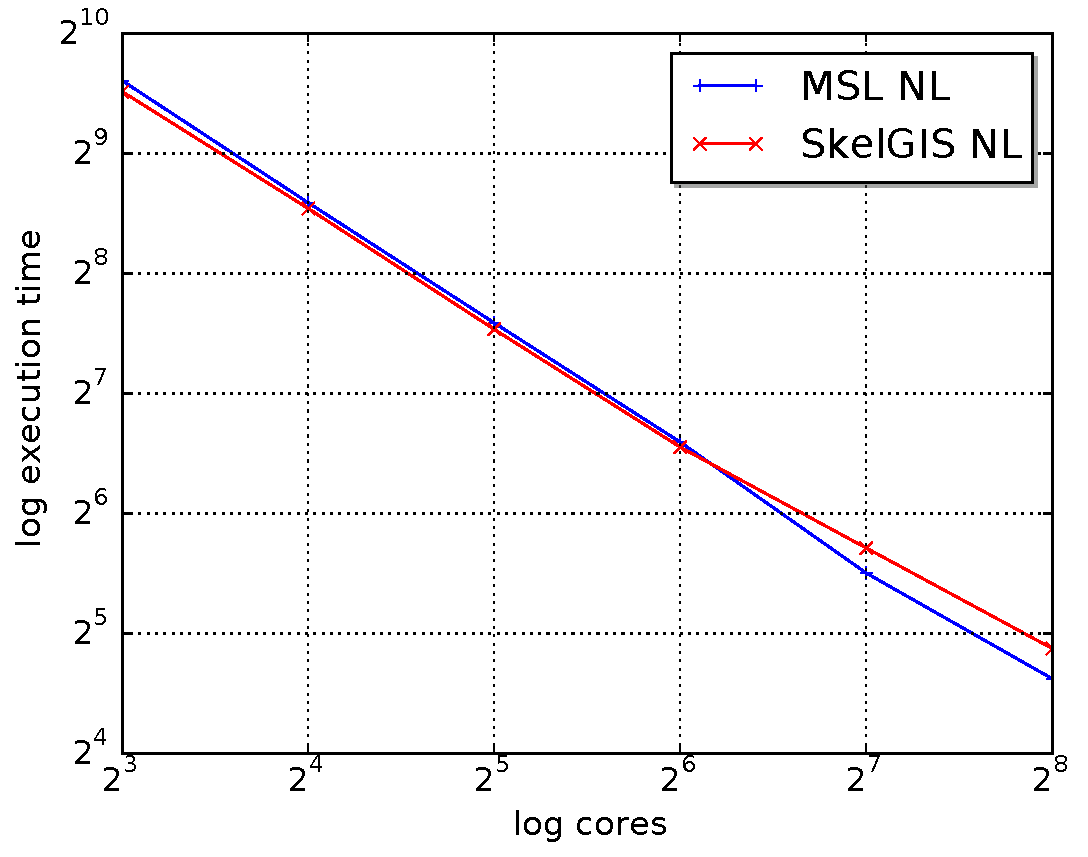
\includegraphics{./images/logtimes_NF.pdf}}
\end{center}
\end{column}
\begin{column}{.5\textwidth}
\begin{center}
\resizebox{\textwidth}{!}{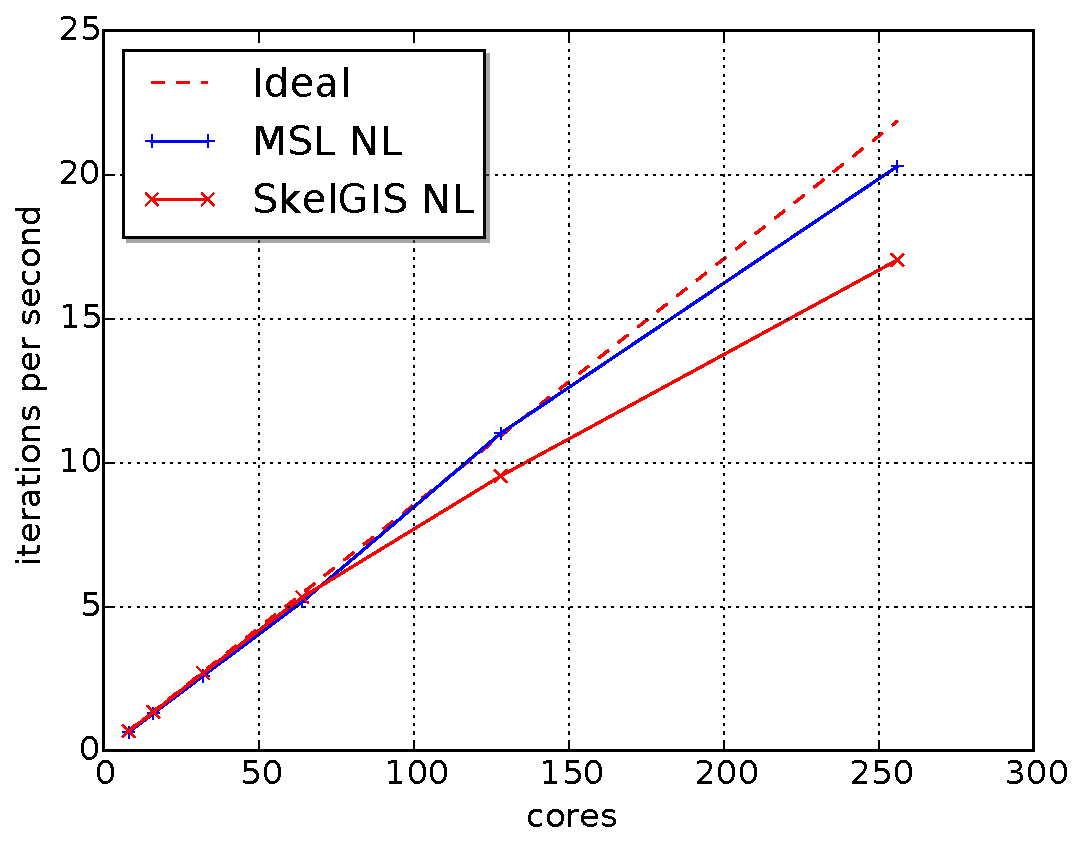
\includegraphics{./images/itpersec_NF.pdf}}
\end{center}
\end{column}
\end{columns}
\end{frame}
%-------------------------------------------------------------

%-------------------------------------------------------------
\section{Conclusion and perspectives}
%-------------------------------------------------------------
\subsection{Conclusion and perspectives}
\begin{frame}
\frametitle{Conclusion}
\begin{block}{Conclusion}
\begin{itemize}
\item A DSL for Multi-Stencil applications (MSL)
\item The compilation of MSL to get a parallel scheduling pattern of the simulation
\begin{itemize}
\item Data parallelism
\item Task parallelism
\end{itemize}
\item The dump to a component-based runtime
\item Data parallelism evaluation: no overhead introduced 
\end{itemize}
\end{block}
\end{frame}
%-------------------------------------------------------------

%-------------------------------------------------------------
\begin{frame}
\begin{block}{Perspectives}
\frametitle{Perspectives}
\begin{itemize}
\item Improvment of the language (convergence criteria, reduction etc.)
\item Scalability up to $32k$ cores on TGCC Curie (CEA)
\item Evaluations on Data+Task parallelism
\begin{itemize}
\item OpenMP 3 inside kernels
\end{itemize}
\item Dynamic scheduling
\begin{itemize}
\item OpenMP 4 with a scheduling component
\item Kstar for StarPU and XKaapi runtimes
\end{itemize}
\item CPU+GPGPUs using stencil compilers (Pochoir, PATUS etc.)
\end{itemize}
$\hookrightarrow$ Show portability, maintainability introduced by components
\end{block}
\end{frame}
%-------------------------------------------------------------

%-------------------------------------------------------------
\begin{frame}
\frametitle{Photos !}
\resizebox{0.9\textwidth}{!}{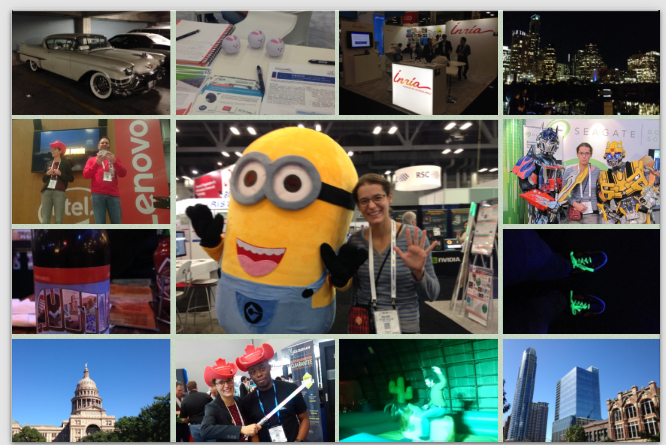
\includegraphics{./images/sc15.jpg}}
\end{frame}
%-------------------------------------------------------------

%\begin{withoutheadline}
% \begin{frame}{}
% \begin{center}
% \huge Thank You !
% \end{center}
% \end{frame}
%\end{withoutheadline}

\end{document}

